\chapter{Literature review}

\section{Deformation modes}
HCP metals, such as $\alpha$ titanium and zirconium, exhibit complex plastic deformation behaviour which is a direct consequence of the intrinsic anisotropy of their low-symmetry crystal structure.
In contrast to FCC metals which have 12 independent and evenly distributed slip systems which can facilitate homogenous deformation for any arbitrary shear, HCP metals rely on a more restricted set of slip systems with widely varying critical resolved shear stresses (CRSS).
Many of the HCP slip systems are not independent, meaning the shear strain that they provide can be equivalently facilitated by a linear combination of other slip systems.
The Von-Mises criterion states that 5 independent slip systems are required to facilitate homogenous arbitrary deformation.
In order to satisfy this condition in HCP, more complex modes such as difficult pyramidal $\langle c + a \rangle$ or deformation twinning must be activated.

\begin{figure}[h!]
\centering
  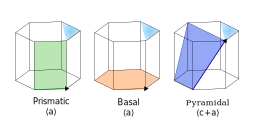
\includegraphics[width=\textwidth]{Figures/slip_systems.pdf}
  \caption{Dominant slip modes in hcp metals.\label{fig.hcp-deformation}}
  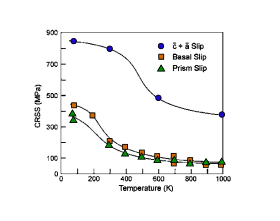
\includegraphics[width=\textwidth]{Figures/CRSS_plot.pdf}
  \caption{Critical resolved shear stresses in Ti-6.6Al single crystal\cite{lütjering2013titanium}.\label{fig.CRSS} }
\end{figure}

\subsection{Slip}
The most favourable slip occurs along crystal planes with the highest atomic packing density.
For a HCP structure with an ideal $c/a$ ratio, this would be the basal \hkl(0002) plane, however in both titanium and zirconium the $c/a$ ratio is less than the ideal value of 1.633, being 1.587 and 1.593 respectively.
This compacted HCP structure results in the highest atomic density on the prismatic planes \hkl{1 0 -1 0}, followed closely by the basal plane \hkl(0002).
The slip direction on both of these planes occurs along the $\langle a \rangle$ direction \hkl<1 1 -2 0>.
Because the Burgers vector of both of these slip families is shared, they cannot provide any shear strain that has a $\langle c \rangle$-axis component.
If one considers a loading along the $\langle c \rangle$-axis, the Schmid factor for both basal and prismatic slip would be zero, meaning plastic deformation must come from another slip mode from a plane that necessarily has a lower atomic density.
The slip mode that activates in this case is the pyramidal $\langle c + a \rangle$, on the \hkl{1 0 -1 1} plane along the \hkl<1 1 -2 3> direction which is the sum of the $\langle c \rangle$ and $\langle a \rangle$ basis vectors.
\fref{fig.CRSS} compares the CRSS values for these three major slip modes as a function of temperature in a Ti-6.6Al single crystal. 
The vast difference in CRSS between the $\langle a \rangle$ and $\langle c + a \rangle$ slip modes results in the heavily anisotropic plastic behaviour of HCP metals.
The crystal orientation of a grain therefore becomes one of the most important factors determining how it will deform, since this will dictate which of the slip modes will be active and what the resolved shear stress will be.



\subsection{Twinning}
Deformation twinning offers an alternative way for the crystal structure to accommodate $\langle c \rangle$-axis strain and is often the favourable mode due to the high CRSS of pyramidal $\langle c + a \rangle$ slip.
The available twinning modes are listed in \tref{table.twin-modes}, which are classified into tensile and compression type twins based on the $\langle c \rangle$ component of the shear.
Twinning is a coordinated reorientation of the lattice and has a distinct orientation relationship with the parent crystal, which can be defined in terms of an angle-axis representation, also listed in \tref{table.twin-modes}.
All of these twin modes result in a tilting of the $\langle c \rangle$-axis, this means that the resulting crystal within the twin volume will be quite distinct from its parent material in terms of plastic response.
For example, for loading along the $\langle c \rangle$-axis a grain will initially be quite hard. If the Type I tensile twin activates, the resulting region will have its $\langle c \rangle$-axis tilted by 85°, resulting in quite a soft orientation that is well aligned for prismatic slip.

%\ Table of twinning modes and their 
\begin{table}[h]
  \vspace{\baselineskip}
  \centering
  \begin{tabular}{l c c c}
    \hline
    \rowcolor{gray!10}
    \textbf{Twinning mode} & $\mathbf{K_1}$   & \textbf{Angle – axis}                       & $\varepsilon$ \\
    \hline
    Tensile Type I         & $\{10\bar{1}2\}$ & $85^\circ \langle 11\bar{2}0 \rangle$       & 0.171         \\
    Tensile Type II        & $\{11\bar{2}1\}$ & $35^\circ \langle 1\bar{1}00 \rangle$       & 0.629         \\
    Compression Type I     & $\{11\bar{2}2\}$ & $65^\circ \langle 1\bar{1}00 \rangle$       & 0.221         \\
    Compression Type II    & $\{10\bar{1}1\}$ & $54^\circ \langle \bar{1}2\bar{1}0 \rangle$ & 0.101         \\
    \hline
  \end{tabular}
  \caption{Twinning systems with twin plane, axis-angle representation, and twinning shear $\varepsilon$. (Nervo. 2016)}
  \label{table.twin-modes}
\end{table}

Unlike slip, deformation twinning has limited activity and eventually becomes exhausted.
In HCP metals, twinning occurs in the early stages of plasticity where it plays a large role in accommodating $\langle c \rangle$-axis strain in grains that are poorly aligned for prismatic slip.
After twin nucleation and growth, eventually the twins consume the majority of their initial grains and subsequent plasticity can continue through dislocation slip.

Deformation twinning adds to the complexity of HCP metals since twin boundaries act as barriers to dislocation motion and secondary twins can form within the primary twin volume.
An accurate description of the deformation behaviour of HCP metals must take all of this into account.

\section{Texture development}
Conventional processing of HCP alloys always produces strong crystallographic texture.
In the case of $\alpha$-titanium and zirconium which have a similar $c/a$ ratio, the particular texture that develops during cold rolling is a basal texture with a split toward the transverse direction of $\pm 25-35^\circ$.
Texture develops during cold working because of the significant crystallographic reorientation that is associated with deformation twinning.
The roller imposes a compressive stress normal to the plane of the plate, but due to the Poisson effect there is a tensile stress in the plane of the plate.
Both compressive (Type I) and tensile (Type I and II) twins have been observed to activate under cold rolling conditions \cite{bozzoloMisorientationsInducedDeformation2010}.
The twinning activity during the early stages of plasticity cause a significant initial texture change, and then subsequent plastic slip may cause further crystallographic reorientation.
Unlike twinning which causes an immediate reorientation, slip results in a gradual rotation.
Prismatic slip, which is the most active slip mode, results in a rotation about the $\langle c \rangle$-axis, while basal and pyramidal $\langle c + a \rangle$ cause the $\langle c \rangle$-axis to tilt.

The final texture that is present after cold rolling is inherited by the recrystallised microstructure, possibly due to preferential nucleation within the twinned regions.
The exact processing route and parameters effect the final resulting texture, but the fact remains that conventional processing of these alloys always results in a strong crystallographic texture.


\section{Polycrystal neighbourhood effects}
\subsection{Slip transfer}
\subsection{Strain networks}

\section{Crystal plasticity modelling}